\chapter{Developing the Processing Tools}
\label{appendix:tools}

Development has been a very iterative process, and has been primarily driven by testing requirements (see \autoref{appendix:testing}). Many of the core functions began as simple proof-of-concepts. As the codebase grew, it underwent significant refactoring. As this is my first major development project, I had to learn---the hard way---how to properly structure a project of this nature. I arrived at many key design principles quite late; some pieces of the project, consequently, were rewritten multiple times. Simultaneously, testing necessitated better ease of use and increased functionality; many features, such as the command line interface to the tools, were added as the need arose and better code organization made implementation possible. With the code as it currently stands, I believe my tools are just as easy to use as GDAL.\footnote{Which, quite honestly, is probably not that easy for most, but should be manageable for anyone with command line experience.}

\section{Review of the classification process}

To reiterate, classifying imagery is a multi-step process. To do so is roughly as follows:

\begin{Spacing}{1.2}
\begin{enumerate}
  \item Build a multi-date image stack or time series image (TSI) from single-date images.
  \item Find “pure” or mostly “pure” TSI pixels (eliminate mixels).
  \item Obtain a reference temporal signature for each of the crops to be identified in TSI.
  \item Run the fit algorithm using the phenological reference curves to generate RMSE rasters for each of the input reference signatures.
  \item Use the threshold tool to find the optimal RMSE threshold for each of the RMSE rasters (requires ground truth data for accuracy assessment). This process outputs the final classified image.
\end{enumerate}
\end{Spacing}

Steps 1, 3, 4, and 5 have been abstracted into individual command line tools, each of which is detailed below. Step 2 is currently a manual process, the procedure for which is detailed in section [TODO: LINK TO METHODS SECTION DISCUSSION ON MIXELS]; how this step was established is explained in \autoref{appendix:testing:r2}. A few other command line tools, such as to plot signatures or to create masked rasters, were also developed, but are not described here. See the project source and documentation on the github site: https://github.com/jkeifer/pyHytemporal. [TODO: SHOULD THIS BE INCLUDED? I HAVE NOT YET BEGUN WRITING THE DOCUMENTATION, AND WHILE I'D LIKE TO, IT IS POSSIBLE THAT IT WILL NOT HAPPEN]

\section{Creating Time Series Images}
\label{appendix:tools:build}

Before I could complete any testing, I had to first determine a way to create a chronological multi-date image stack---a time series image (TSI)---in which the values of each pixel represent the temporal signature of its contents. A TSI can be thought of as the temporal equivalent of a hyperspectral data cube, and is the primary data structure used in the analysis.

Despite the fancy terminology, however, a TSI (or hyperspectral data cube, for that matter) is merely a multi-band raster file, where each band is the data from a given date (or for a spectral band, in a data cube). Abstracting this concept a step further, a raster file is simply an array. A single-band raster is therefore a two-dimensional array where the columns and rows of the image are represented by the columns and rows of the array, and the data are single-dimension values in each cell. Adding multiple bands, or in this case dates, to the image is easily accomplished by adding another dimension to the array.

The Python Geographic Data Abstraction Library (GDAL) and numpy libraries include objects and methods which make opening spatially-enabled raster files as arrays, saving arrays to spatially-enabled raster files, and manipulating arrays in memory trivial tasks. Thus, creating a tool to build a TSI from a selection of single-date raster files was straightforward and easy, and did not require any extensive or involved testing.

The finished tool, which I call the Build Multidate Image tool, simply requires the user to specify a director containing the MODIS .hdf files that will be assembled into a TSI. The the name of the VI the tool should extract from the .hdf files is an optional argument, as the tool defaults to extracting the NDVI raster data.

\section{Extracting Reference Temporal Signatures}
\label{appendix:tools:extract}

While I hope in the future libraries of temporal signatures will allow researchers to use temporal classification tools without needing to derive their own signatures, obviously such resources are not available now. For my work this necessitated that I devise a tool to create such signatures. I named this tool the Extract Signatures Tool (EST).

I decided, in order to maximize ease of use, the tool would need to accept a set of points as an input, find the pixel coordinates in the TSI for each point, then extract each point’s temporal signature. The average of these signatures could be calculated then written to a file for later use.

To implement this solution, I created a library to read point features from shapefiles, and wrote a function to take the geographic coordinates of each point in a shapefile and convert them into a list of pixel coordinates in a specified image. Next, I wrote a set of functions to read the values of such a list of pixel coordinates and write them to a text file with the format shown in \autoref{fig:reffile}. Then, I created a function to find the mean of each date, writing the result to another file. Each of the created files was in plain-text ASII format, and I decided to use the file extension .ref.

I based the formatting of the .ref files on the .sig files used by ENVI for hyperspectral signatures. Using a plain-text file-based data format currently seems to be the best solution for storing reference signatures, as the data are very simply structured and files are highly portable. However, future implementations of the EST may benefit from a more rigid or better contained data format.

\begin{ssfigure}
  \centering
  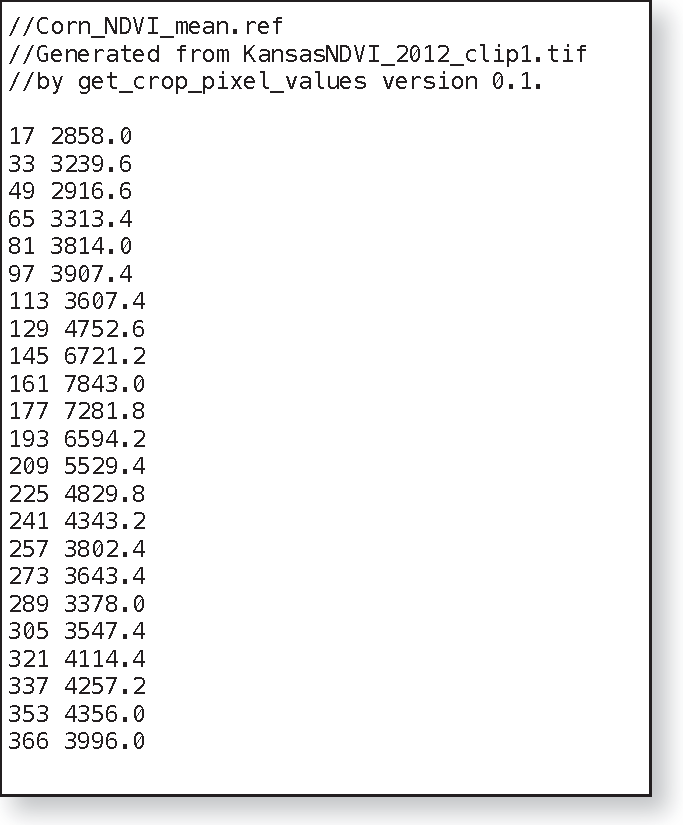
\includegraphics[scale=0.75]{Graphics/reffile.pdf}
  \caption{An Example .ref File Used to Store Reference Temporal Signatures}
  \medskip
  \small
  Comments are marked by // and each non-comment row represents a VI value (right column) for a given DOY (left column), separated by a space.
  \label{fig:reffile}
\end{ssfigure}



\section{The Fit Algorithm}
\label{appendix:tools:fit}

Developing the fit algorithm and the corresponding tool was a more complex problem. As described in \autoref{chapter:methods:phenology-fitting}, the basis of the algorithm is \autoref{eq:1}. The equations finds the average difference between a pixel signature and a reference signature (the RMSE), while allowing the reference be transformed within predefined bounds. Minimizing the equation enables the degree of fit between a reference signature and a pixel signature to be quantified. To implement the algorithm, I decided to use scipy’s minimize function. I began by building the simplest implementation possible, while making as many parameters as possible into arguments of the enclosing function to allow future testing. I continued building out the functionality until I had a tool capable of reading in a TSI from a file path and reference temporal signature .ref files in a directory. The tool would then process the TSI using the .ref files, and output a RMSE raster corresponding to each .ref file. The value of a pixel in a RMSE raster is the RMSE value of the reference temporal signature fit to the TSI pixels.

One clear problem early on was speed. Python’s global interpreter lock (GIL), intended to increase the security and reliability of running python code, also has the consequence of limiting code execution to a single processor core. With current multicore processor designs, this prohibits python from using much of the available processing resources. For example, in my eight-core computer, I was limited to using only 12.5 percent of its processing capabilities.

To get around this, I redesigned the tool to allow the use of the python multiprocessing module. With multiprocessing, I was able to spawn a new worker process for each reference signature used (limited to a maximum number of processes as specified by the user), devoting an entire core to processing each RMSE raster. At first, this seemed to be a great solution: when using five reference signatures, I could produce the RMSE raster for all five in one-fifth the time. However, the parallel use of resources is not as straightforward as it seems.

In the later stages of testing, I began getting a serious error when attempting to generate the RMSE rasters. I am unsure why the problems began; it may be related to refactoring the code. I know that it had not occurred in earlier testing as the issue resulted in a fatal error, where the program would try to read in a pixel from the TSI and would get a null value. Strangely, this issue would always happen on the twentieth row of the TSI. Even stranger, printing the pixel value to the screen would not get a null value, and the program would continue, but careful investigation revealed that the value returned from problem pixels would not be valid (often being zero for every band, or a repeating pattern of negative numbers).

I tried eliminating the parallelism problem by using just a single worker process, to test the same code but with only a single process trying to access the GDAL image object in memory. Preventing concurrent access to that object had the intended effect, and the problem disappeared. I tried using the multiprocessing lock construct to prevent multiple processes from reading the image object simultaneously, but this had no effect. Finally, after reading the multiprocessing documentation yet again, I decided I would try reading the TSI into an array in memory, as arrays seemed to be safer in concurrent applications. With this change, the problem vanished. Additionally, this solution also had the benefit of providing a moderate speed boost, though unfortunately this solution also raises the memory requirements of the program: the entire TSI must be read into memory, and all the arrays for the output RMSE rasters are also in memory, so the memory footprint is roughly equal to $s(n + 1)$ where $s$ is the size, in bytes, of the TSI image, and $n$ is the number of worker processes.

Other problems I had throughout development were issues involving pixel coordinates. Sometime highly pervasive, these problems stemmed from the fact that arrays use matrix-style coordinates in row-column order, while GDAL functions require coordinates in terms of x-offset and y-offset, which is actually column-row order\footnote{One piece of advice to anyone developing raster tools: do not use square test rasters. Doing so hides many such bugs. For example, if the pixel coordinates are accidentally supplied in row-column format when a function is expecting column-row order, a square image will never throw an error, whereas a rectangular image will result in an error when the index of the array is out of bounds. Many otherwise subtle programming errors can be caught this way.}. One must remain cognizant of the data type with which he or she is interacting, especially when refactoring changes between GDAL image objects and arrays, or vise versa.

Using the algorithm is easy, as it has a command line interface through the Find Fit Tool. Due to the numerous parameters required by the algorithm, the command has many options. However, it only requires that the user specify the the path to the TSI image, the path to the directory containing the .ref reference signature files, and the start day-of-year and day-of-year interval for the TSI. All of the other options require user input only if the user wants to use a non-default value.

\section{Creating a Classification From the RMSE Rasters}
\label{appendix:tools:classify}

Merely finding the RMSE rasters does not a classification make. The first step in creating a classification is to find useable RMSE values; even pixels that are obviously different than a reference signature will result in a RMSE value. Thus, the RMSE rasters need to be thresholded to eliminate high RMSEs.

Choosing a value at which to threshold the RMSE rasters is not a simple decision. One can think of the threshold in a similar manner to weighting: a higher RMSE threshold will allow more pixels from that RMSE raster to be considered in the final classification. The correct threshold for a RMSE raster will vary depending on a variety of factors, including what types of crops are in the sample area, what crops are trying to be identified, and how homogeneous the pixels for that crop are in comparison to the reference signature used. The extent to which these and other factors influence the optimal threshold is not well understood and requires further study. Despite not knowing the exact effects of these factors on the optimal threshold value, it is clear that the optimal value will vary between RMSE rasters. That is, a single value used across all RMSE rasters in a classification is unlikely to provide the highest possible accuracy.

Once the RMSE rasters are thresholded, one can make a classification by finding the best fit for every pixel. For example, if a given pixel had thresholded RMSE values for corn, soy, and wheat of 356.7, 531.5, and none (as the original RMSE was above the threshold used), respectively, the best fitting signature would be corn, and the pixel could be classified as corn. If a pixel did not have any RMSE values under the threshold used, then that pixel would not be classified (a classification as ``other'' would be equally correct).

In order to automate this thresholding/best fit process, and to provide a means to quickly iterate through possible RMSE threshold combinations, I created a command line tool called the Classify Tool. The tool requires the user to specify the RMSE rasters to be classified, a truth raster, and RMSE threshold parameters. The threshold parameters allow the user to specify the starting RMSE threshold value, the number of RMSE threshold steps to test, and a RMSE threshold step value (how much to increase the threshold each step). The truth raster is ground truth for the entire classified area, and is assumed to match the RMSE rasters’ pixel grids exactly and cover the same geographic extent (such that every pixel coordinate in the RMSE rasters and truth raster will describe the same geographic location and extent). From these parameters, the tool will automatically generate every possible threshold combination. Then, the tool will brute force through those combinations, creating a classification with each and checking the accuracy against the truth raster. Once completed, the tool will output a classification raster created with the highest accuracy combination, as well as a report detailing every combination tested with a confusion matrix for each.